% Provenance (never printed): see sources/outline_sources.md (Year 3: primordial
% nucleosynthesis and stellar burning recalled from the physics books; the s and r
% processes; supernovae and neutron-star mergers; galactic chemical evolution; from the
% solar abundances to the composition of the Earth).
% Brief: sources/book5/BRIEFS.md, ch. 30. Curves from figdata/bachelor-3/
% solar_abundances.py (Asplund, Amarsi and Grevesse 2021, Table 2), neutron_capture.py
% (their Table B.1 isotopes, KADoNiS v0.3 cross sections, IAEA Live Chart half-lives) and
% chemical_evolution.py (closed box against the Geneva-Copenhagen survey of Casagrande et
% al. 2011, and a two-phase [alpha/Fe] model). Exercise and problem values in the Book 5
% scratch calculator calc/ch30.py.
\chapter{De onde vêm os elementos}\label{ch:b3:origin-of-elements}

O cálcio de um penhasco calcário foi produzido, em sua maior parte, no interior
de estrelas massivas que explodiram antes do nascimento do Sol. O ferro do
núcleo da Terra vem sobretudo de outro tipo de explosão, a de uma
anã branca. A platina de um anel pertence a um pico de abundância construído
por surtos de \omterm{def:b3:origin-of-elements:s-process}{captura de nêutrons} que duram segundos, em coalescências de duas estrelas de
nêutrons ou em um tipo raro de supernova; qual dos dois produziu a maior parte
dele ainda é objeto de debate.
Cada um desses eventos deixou sua marca na composição do Sol,
que é também, com exceção dos poucos elementos que os planetas não
conseguiram reter, a composição do Sistema Solar. Este capítulo lê esse
registro: apresenta as \omterm{def:b3:origin-of-elements:abundance}{abundâncias solares}, recorda como os elementos leves
foram formados, acompanha as \omterm{def:b3:origin-of-elements:s-process}{capturas de nêutrons} que construíram os pesados, identifica
os locais onde cada processo ocorre, e modela como a composição de uma
galáxia muda à medida que suas estrelas nascem e morrem. Termina onde a geologia dos
volumes anteriores começa: por que a Terra, feita do mesmo material que
o Sol, é tão rica em ferro e tão pobre em voláteis.
% ledger: matteucci21:production, cowan21:rprocess, kobayashi20:origins, asplund21:fig1

\begin{recall}
A nucleossíntese do Big Bang, a fusão de hidrogênio e hélio em estrelas,
a energia de ligação por núcleon e seu máximo perto do ferro, o vale da
estabilidade, o decaimento beta e as meias-vidas, a seção de choque de uma reação,
estrelas da sequência principal, gigantes vermelhas, anãs brancas, estrelas de nêutrons e
supernovas estão nos livros de física. As classes de meteoritos, os condritos CI,
a temperatura de condensação, os elementos refratários e voláteis, as classes de Goldschmidt
e a Terra silicática global estão no
volume do segundo ano, em seus capítulos sobre a formação dos planetas e sobre
os elementos da Terra. A estrutura da Galáxia, seus discos fino e
espesso, seu halo e suas populações estelares estão no capítulo
anterior.
\end{recall}

\section{As abundâncias solares}\label{sec:b3:origin-of-elements:solar}

O Sol detém mais de \qty{99.85}{\percent} da massa do Sistema
Solar, e suas camadas externas conservaram, à exceção de alguns elementos leves
e de uma lenta sedimentação dos mais pesados, a composição do gás a partir do qual
se formaram o Sol e os planetas. Sua composição é lida de duas maneiras:
pelas linhas de absorção de sua fotosfera e pelos condritos CI,
os meteoritos cuja composição, exceto pelos elementos mais voláteis,
elementos, é a mais próxima de todos os materiais conhecidos da do Sol.
% ledger: asplund21:fig1, asplund21:ci

\begin{definition}[Abundância solar; dex]\label{def:b3:origin-of-elements:abundance}
A \emph{abundância solar}\index{abundância solar} de um elemento $X$ é
o número de seus átomos em relação aos de hidrogênio no Sol,
expresso em escala logarítmica na qual o hidrogênio é fixado em $12$:
\[
\log\varepsilon(X) = 12 + \log_{10}\frac{N_X}{N_\mathrm{H}} .
\]
Uma diferença de uma unidade em tal logaritmo chama-se um
\emph{dex}\index{dex}: duas abundâncias que diferem de $0.3$~dex diferem por
um fator $10^{0.3} \approx 2$. Para uma estrela, a abundância relativa ao
Sol escreve-se com colchetes,
$[X/\mathrm{H}] = \log_{10}(N_X/N_\mathrm{H})_\star -
\log_{10}(N_X/N_\mathrm{H})_\odot$, e analogamente $[X/Y]$ para quaisquer dois
elementos.
\end{definition}

A figura abaixo mostra as \omterm{def:b3:origin-of-elements:abundance}{abundâncias solares} da compilação recente
que reavaliou todos os 83 elementos de vida longa. O ferro, com
$\log\varepsilon = 7.46$, tem um átomo para cada \num{34700} átomos de
hidrogênio; o hélio tem \num{0.0820} átomo por átomo de hidrogênio. Vários
traços se destacam, e o restante do capítulo os explica.
% ledger: asplund21:abstract, asplund21:ci, data:b5-asplund21

\begin{omfigure}
\centering
\begin{tikzpicture}
\begin{axis}[width=0.95\linewidth, height=8.4cm, xmin=0, xmax=94,
  ymin=-1.8, ymax=12.8, xlabel={número atômico $Z$},
  ylabel={$\log\varepsilon(X)$ \;($\log\varepsilon(\mathrm{H}) = 12$)},
  tick label style={font=\scriptsize}, label style={font=\small},
  legend style={font=\scriptsize, at={(0.5,-0.17)}, anchor=north,
    legend columns=2, draw=none, cells={anchor=west},
    /tikz/every even column/.append style={column sep=1em}}]
\addplot[blue!70!black, mark=*, mark size=1.3pt, restrict x to domain=0:84]
  table[x=Z, y=logeps] {figdata/out/bachelor-3-solar_abundances-even.dat};
\addlegendentry{$Z$ par}
\addplot[blue!70!black, mark=*, mark size=1.3pt, restrict x to domain=88:94, forget plot]
  table[x=Z, y=logeps] {figdata/out/bachelor-3-solar_abundances-even.dat};
\addplot[red!70!black, mark=o, mark size=1.4pt]
  table[x=Z, y=logeps] {figdata/out/bachelor-3-solar_abundances-odd.dat};
\addlegendentry{$Z$ ímpar}
\begin{scope}[font=\scriptsize]
\node[anchor=west] at (axis cs:2.2,12.2) {H};
\node[anchor=west] at (axis cs:3.0,10.9) {He};
\node[anchor=west] at (axis cs:5.6,1.0) {Li, Be, B};
\node[anchor=south] at (axis cs:8,8.95) {O};
\node[anchor=south] at (axis cs:6,8.6) {C};
\node[anchor=south, align=center] at (axis cs:26,7.75) {Fe\\[-1pt]pico};
\node[anchor=north] at (axis cs:21,2.95) {Sc};
\node[anchor=south, align=center] at (axis cs:38.5,3.05) {Sr--Zr\\[-1pt]($N = 50$)};
\node[anchor=south] at (axis cs:51.5,2.5) {Te, Xe (r)};
\node[anchor=south, align=center] at (axis cs:58.5,3.7) {Ba\\[-1pt]($N = 82$)};
\node[anchor=south] at (axis cs:76.5,1.95) {Pt (r)};
\node[anchor=south, align=center] at (axis cs:82.5,2.85) {Pb\\[-1pt]($N = 126$)};
\node[anchor=south] at (axis cs:89.6,0.15) {Th};
\node[anchor=north] at (axis cs:92,-0.7) {U};
\end{scope}
\end{axis}
\end{tikzpicture}
\par\smallskip{\small As abundâncias dos elementos no Sol, em uma
escala logarítmica com o hidrogênio em 12: valores fotosféricos, ou os dos
condritos CI, para os elementos que não possuem
linha fotosférica mensurável (Asplund, Amarsi e Grevesse, 2021). Os números atômicos pares e ímpares
são desenhados como duas linhas. Tecnécio ($Z = 43$) e promécio ($Z = 61$)
não têm isótopo de vida longa, nem os elementos entre bismuto e
tório.}\label{fig:b3:origin-of-elements:curve}
\end{omfigure}
% ledger: data:b5-asplund21, asplund21:fig1

\begin{enumerate}
\item Hidrogênio e hélio formam quase todos os átomos, mil vezes
  mais que todos os outros juntos; ambos foram produzidos no Big Bang, e
  parte do hélio desde então, nas estrelas.
\item Lítio, berílio e boro, logo depois do hélio, situam-se muito abaixo
  do carbono: o berílio é doze milhões de vezes menos abundante.
\item As abundâncias caem acentuadamente do oxigênio até os elementos
  pesados, com picos em torno do oxigênio, do ferro, do bário e do chumbo,
  e picos menores que a figura identifica.
\item Elementos de número atômico par são mais abundantes que seus vizinhos
  ímpares: o escândio, entre o cálcio e o titânio, é cerca de \num{1400}
  vezes mais raro que o cálcio e \num{68} vezes mais raro que o titânio. Esse
  é o \emph{efeito par--ímpar}.
\item Além do pico do ferro, a curva se achata: do ferro até o ouro a
  abundância cai por um fator de \num{3.5e6}, mas do ouro até o chumbo ela
  sobe novamente, por um fator de onze.
\end{enumerate}
% ledger: asplund21:fig1, data:b5-asplund21

Em massa, a fotosfera atual tem $X = 0.7438$ de hidrogênio,
$Y = 0.2423$ de hélio e $Z = 0.0139$ de todo o resto. Corrigidos pelos
elementos pesados que se depositaram abaixo da fotosfera desde que o Sol
se formou, os valores protossolares, aqueles do gás a partir do qual o Sol
nasceu, são $X = 0.7121$, $Y = 0.2725$ e $Z = 0.0154$.
% ledger: asplund21:xyz

\begin{definition}[Metalicidade]\label{def:b3:origin-of-elements:metallicity}
A \emph{metalicidade}\index{metalicidade} de uma estrela ou de um gás é seu
conteúdo de elementos mais pesados que o hélio, chamados metais em astronomia
qualquer que seja sua química: como fração mássica $Z$ ou, como costuma ser
medida, como a abundância de ferro relativa ao Sol, $[\mathrm{Fe/H}]$.
Uma estrela com $[\mathrm{Fe/H}] = -1$ tem um décimo do ferro do Sol
por átomo de hidrogênio.
\end{definition}

As duas fontes das \omterm{def:b3:origin-of-elements:abundance}{abundâncias solares} concordam notavelmente bem. A
figura abaixo as compara elemento a elemento. Para 58 elementos, aqueles
nem muito voláteis para os meteoritos nem destruídos no Sol, a diferença
média ponderada entre a abundância fotosférica e a do CI é
$\num[separate-uncertainty=true]{0.000 \pm 0.007}$~\omterm{def:b3:origin-of-elements:abundance}{dex}. Dois grupos
se afastam da reta. Os meteoritos contêm muito menos hidrogênio, hélio,
carbono, nitrogênio, oxigênio e gases nobres que o Sol: esses elementos
permaneceram no gás quando os sólidos se condensaram. O Sol contém
\num{200} vezes menos lítio que os meteoritos: ele destruiu
\qty{99.5}{\percent} de seu lítio por queima nuclear.
% ledger: asplund21:ci, data:b5-asplund21

\begin{omfigure}
\centering
\begin{tikzpicture}
\begin{axis}[width=0.66\linewidth, height=0.66\linewidth, xmin=-3, xmax=12.8,
  ymin=-1, ymax=12.8, xlabel={$\log\varepsilon$ nos condritos CI},
  ylabel={$\log\varepsilon$ na fotosfera},
  tick label style={font=\scriptsize}, label style={font=\small},
  scatter/classes={0={mark=*, mark size=1.3pt, black!70},
    1={mark=square*, mark size=1.5pt, red!70!black},
    2={mark=triangle*, mark size=2pt, blue!70!black}}]
\addplot[black!40, dashed, domain=-1:12.8, samples=2] {x};
\addplot[scatter, only marks, scatter src=explicit symbolic]
  table[x=ci, y=phot, meta=group] {figdata/out/bachelor-3-solar_abundances-compare.dat};
\begin{scope}[font=\scriptsize, red!60!black]
\node[anchor=east] at (axis cs:8.12,12.0) {H};
\node[anchor=west] at (axis cs:1.45,10.914) {He};
\node[anchor=east] at (axis cs:7.25,8.55) {C};
\node[anchor=east] at (axis cs:6.1,7.83) {N};
\node[anchor=west] at (axis cs:8.5,8.45) {O};
\node[anchor=west] at (axis cs:-0.97,8.06) {Ne};
\node[anchor=west] at (axis cs:-0.35,6.38) {Ar};
\node[anchor=west] at (axis cs:-2.12,3.12) {Kr};
\node[anchor=west] at (axis cs:-1.8,2.22) {Xe};
\end{scope}
\node[font=\scriptsize, blue!60!black, anchor=west] at (axis cs:3.4,0.96) {Li};
\end{axis}
\end{tikzpicture}
\par\smallskip{\small O Sol comparado aos condritos CI: cada ponto é
um elemento com os dois valores (Asplund, Amarsi e Grevesse, 2021; a
escala meteorítica é fixada de modo que o silício concorde). A linha
tracejada é a igualdade. Pontos pretos: os 58 elementos que concordam.
Quadrados: hidrogênio, hélio, carbono, nitrogênio, oxigênio e os gases
nobres, que os meteoritos não reteram. Triângulo: lítio, destruído no
Sol.}\label{fig:b3:origin-of-elements:sun-ci}
\end{omfigure}
% ledger: data:b5-asplund21, asplund21:ci

A concordância é um fato de grande peso para a geologia. Ela significa que
os meteoritos, que podem ser analisados em laboratório, fornecem a
composição do Sistema Solar para todos os elementos, exceto os mais
voláteis; e que o Sol, cuja fotosfera fornece hidrogênio, carbono,
nitrogênio e oxigênio, completa o restante. O volume do segundo ano
construiu sobre essa base a composição da Terra global.
% ledger: asplund21:ci

\section{Os elementos leves e as estrelas}\label{sec:b3:origin-of-elements:stars}

Os livros de física descrevem a nucleossíntese do Big Bang: nos primeiros
três minutos, à medida que o Universo esfriava, prótons e nêutrons se
combinaram em deutério, hélio-3, hélio-4 e um traço de lítio-7, e em nada
mais pesado. As abundâncias primordiais observadas são uma fração mássica
de hélio $Y_\mathrm{p} = \num[separate-uncertainty=true]{0.245 \pm 0.003}$, uma
razão deutério-hidrogênio de \num{2.5e-5} e uma razão lítio-hidrogênio de
\num{1.45e-10}, esta última medida em estrelas antigas pobres em metais do
halo galáctico. Todos os outros elementos, e o excesso de hélio no Sol,
$0.2725 - 0.245 \approx 0.028$, foram produzidos nas estrelas.
% ledger: pdg25:bbn, asplund21:xyz

As estrelas dos livros de física queimam hidrogênio em hélio na sequência
principal, depois hélio em carbono e oxigênio como gigantes vermelhas; as
mais massivas prosseguem, em camadas ao redor de seus núcleos, até neônio,
magnésio, silício e, por fim, ferro. A fusão para aí, porque a energia de
ligação por núcleon é máxima perto do ferro: construir núcleos mais pesados
por fusão absorve energia em vez de liberá-la. Além do pico do ferro, os
elementos são formados por outra via, a \omterm{def:b3:origin-of-elements:s-process}{captura de nêutrons}, assunto da
próxima seção. Lítio, berílio e boro são frágeis: são destruídos nas
temperaturas do interior estelar, o que explica por que o Sol queimou
quase todo o seu lítio e por que esses três elementos formam um vale na
curva de abundância.

\begin{definition}[Elemento alfa]\label{def:b3:origin-of-elements:alpha}
Um \emph{elemento alfa}\index{elemento alfa} é um dos elementos de $Z$ par
oxigênio, neônio, magnésio, silício, enxofre e cálcio, cujos
isótopos mais abundantes ($^{16}\mathrm{O}$, $^{20}\mathrm{Ne}$,
$^{24}\mathrm{Mg}$, $^{28}\mathrm{Si}$, $^{32}\mathrm{S}$,
$^{40}\mathrm{Ca}$) têm números de massa que são múltiplos de quatro, e
que são produzidos principalmente em estrelas massivas e devolvidos ao gás por sua
explosão como supernovas de colapso do núcleo.
\end{definition}
% ledger: matteucci21:production, data:b5-asplund21

Os picos do oxigênio e dos \omterm{def:b3:origin-of-elements:alpha}{elementos alfa}, e o efeito par--ímpar,
são as marcas dessas etapas de queima: núcleos de hélio são incorporados aos
núcleos pares com mais facilidade do que os ímpares, e núcleos
com número par de prótons são mais fortemente ligados. O que uma estrela devolve
ao gás depende de sua massa.

\begin{definition}[Rendimento estelar]\label{def:b3:origin-of-elements:yield}
O \emph{rendimento estelar}\index{rendimento estelar} de um elemento proveniente de uma estrela
de massa inicial dada é a massa desse elemento que a estrela produziu
e devolve ao gás interestelar, em ventos e em sua
explosão final, como fração da massa da estrela.
\end{definition}
% ledger: matteucci21:yield

Estrelas de menos de \qty{0.8}{M_\odot} vivem mais do que a idade do
Universo e não devolvem nada. Estrelas de \num{0.8} a \qty{8}{M_\odot}
devolvem hélio, nitrogênio, carbono e os elementos pesados do \omterm{def:b3:origin-of-elements:s-process}{processo s}
(bário, ítrio, estrôncio) em seus ventos, e terminam como
anãs brancas de carbono--oxigênio. Estrelas de mais de \num{8} a \qty{10}{M_\odot} produzem
principalmente os \omterm{def:b3:origin-of-elements:alpha}{elementos alfa} e algum ferro, e explodem como
supernovas de colapso do núcleo. Uma anã branca em binária próxima pode explodir como uma supernova do tipo~Ia,
e essas explosões produzem a maior parte do ferro.
% ledger: matteucci21:production

\begin{omfigure}
\centering
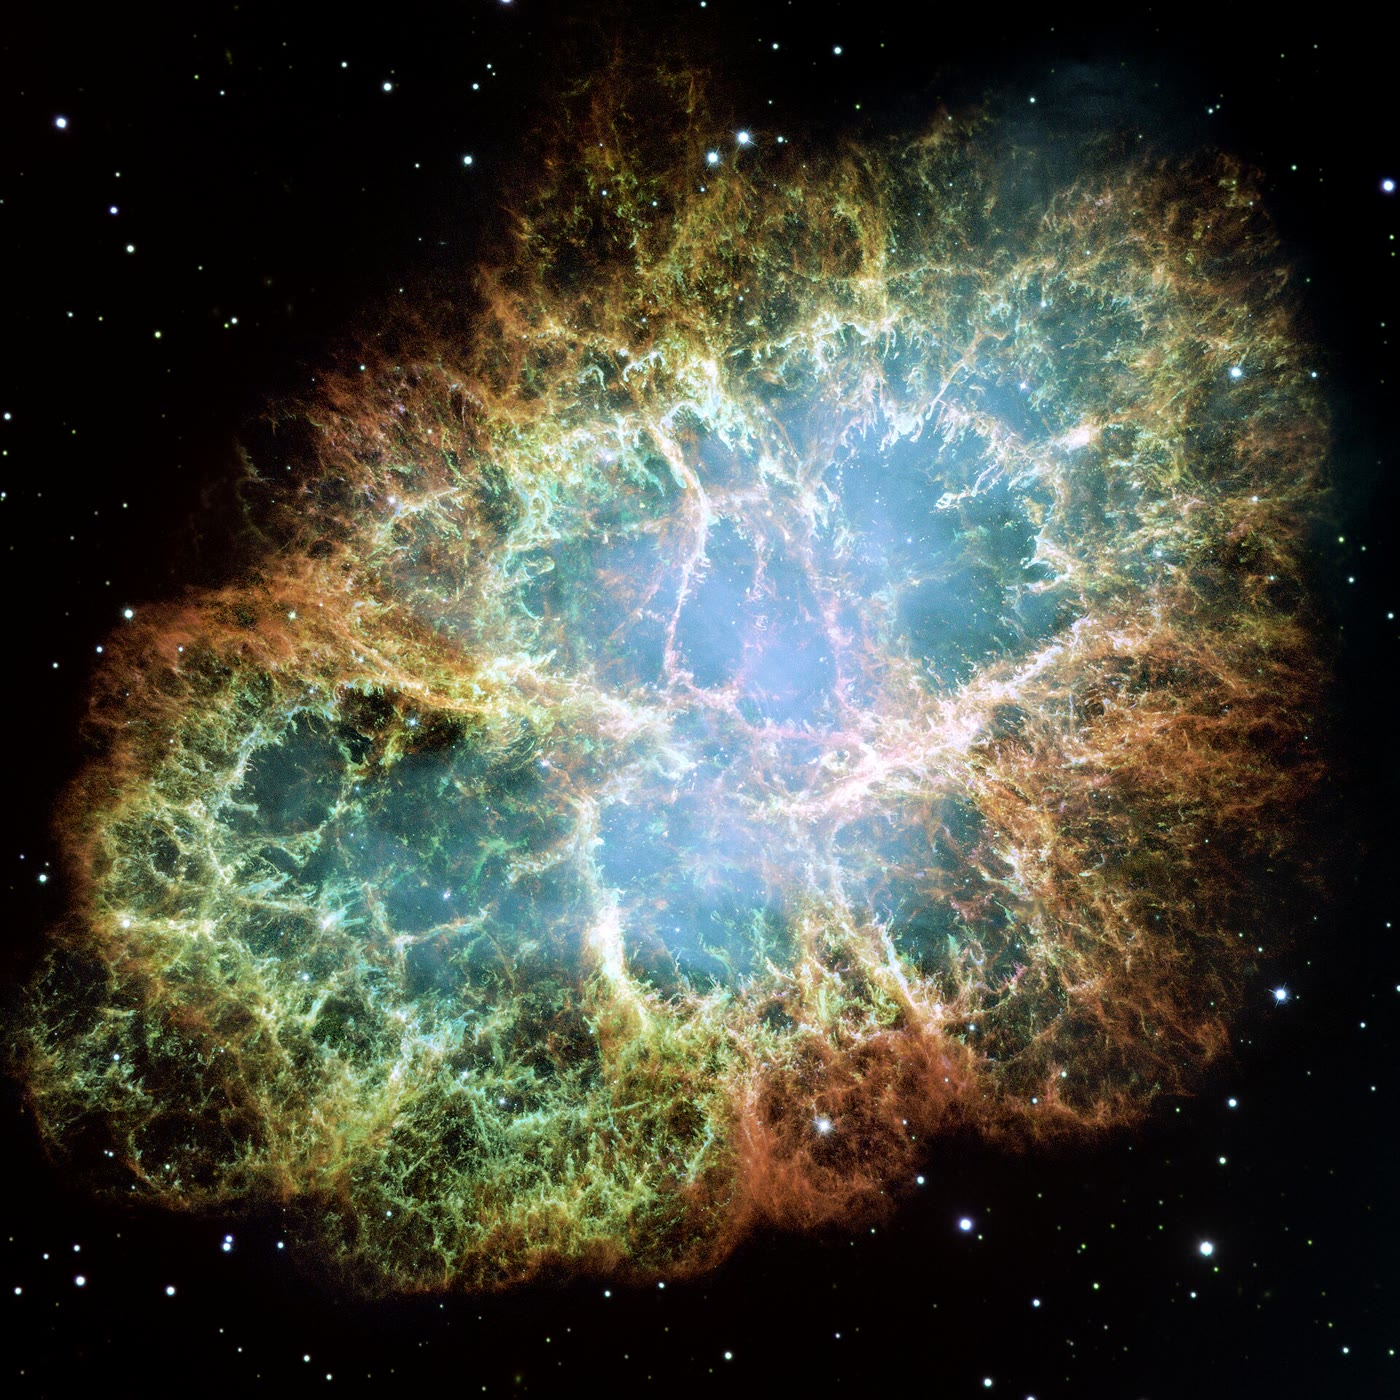
\includegraphics[width=0.5\linewidth]{images/book5/b3-crab-nebula.jpg}
\par\smallskip{\small A Nebulosa do Caranguejo, um mosaico de 24 exposições do Hubble Space
Telescope: os restos em expansão de uma estrela cuja explosão
foi registrada por astrônomos japoneses e chineses em 1054. Os filamentos laranja
são as camadas externas esfarrapadas da estrela, em sua maior parte hidrogênio; o brilho azulado
interno vem de elétrons em espiral ao redor das linhas do campo magnético
da estrela de nêutrons no centro, que gira trinta vezes por
segundo. O gás dos filamentos, que carrega o que a estrela produziu, mistura-se
ao meio interestelar. NASA, ESA, J.~Hester e A.~Loll, domínio
público.}\label{fig:b3:origin-of-elements:crab}
\end{omfigure}
% ledger: photo:b3-crab-nebula

\section{Captura de nêutrons}\label{sec:b3:origin-of-elements:neutrons}

Um nêutron não tem carga elétrica e não é repelido por um núcleo: até
um nêutron lento entra nele, e o núcleo, agora com uma unidade de massa a mais, libera
a energia de ligação como raio gama. Capturas repetidas produzem
isótopos mais pesados do mesmo elemento até que um deles seja instável; ele então decai,
geralmente por decaimento beta-menos, no elemento seguinte, que captura
por sua vez. Quais núcleos são formados depende de uma comparação: o tempo entre
duas capturas e a meia-vida dos núcleos instáveis encontrados no
caminho.

\begin{definition}[Captura de nêutrons; processo s; processo r]\label{def:b3:origin-of-elements:s-process}
A \emph{captura de nêutrons}\index{captura de nêutrons} é a absorção de um
nêutron livre por um núcleo, $(Z, A) + \mathrm{n} \to (Z, A+1) + \gamma$.
No \emph{processo s}\index{processo s} (lento), as capturas
são mais lentas do que a maioria dos decaimentos beta: o tempo entre duas capturas em um
mesmo núcleo é de centenas a milhares de anos, de modo que um núcleo instável
quase sempre decai antes de poder capturar, e a cadeia de capturas
e decaimentos segue o vale da estabilidade. No
\emph{processo r}\index{processo r} (rápido), a densidade de nêutrons
é tão alta que as capturas são muito mais rápidas do que os decaimentos: os núcleos são
levados a isótopos muito ricos em nêutrons, longe da estabilidade, em poucos
segundos, e decaem de volta à estabilidade quando os nêutrons se esgotam.
\end{definition}
% ledger: cowan21:timescales, cowan21:rprocess, kaeppeler11:overview

Os dois processos atingem núcleos diferentes, e a carta de nuclídeos
mostra quais. A figura abaixo desenha uma faixa dela, do cádmio ao
bário. O \omterm{def:b3:origin-of-elements:s-process}{processo s} a percorre acompanhando o vale da estabilidade: ao longo
de uma linha de um elemento enquanto os isótopos são estáveis, depois sobe uma linha por um
decaimento beta. O \omterm{def:b3:origin-of-elements:s-process}{processo r} vem do lado rico em nêutrons, embaixo
à direita: cada núcleo muito rico em nêutrons decai por sucessivos decaimentos beta-menos
ao longo de seu isóbaro, mantendo o número de massa, e para no primeiro
núcleo estável que encontra. Um núcleo estável que tem um isóbaro estável de
$Z$ menor é \emph{blindado} do \omterm{def:b3:origin-of-elements:s-process}{processo r}: $^{122}\mathrm{Te}$
fica atrás de $^{122}\mathrm{Sn}$, $^{123}\mathrm{Te}$ atrás de
$^{123}\mathrm{Sb}$, $^{124}\mathrm{Te}$ atrás de $^{124}\mathrm{Sn}$.
Esses três só podem ser formados pelo \omterm{def:b3:origin-of-elements:s-process}{processo s}: são
\emph{somente-s}. Inversamente, $^{128}\mathrm{Te}$ e $^{130}\mathrm{Te}$
ficam além do caminho s, o que deixa o telúrio no $^{127}\mathrm{Te}$,
cuja meia-vida é \qty{9.35}{h}: são somente-r.
% ledger: kaeppeler11:overview, data:b5-iaea-gs, data:b5-sigman

\begin{omfigure}
\centering
\begin{tikzpicture}
\begin{axis}[x=0.62cm, y=0.7cm, xmin=61.4, xmax=84.6, ymin=47.4, ymax=56.6,
  xlabel={número de nêutrons $N$}, ylabel={},
  xtick={62,64,...,84}, ytick={48,...,56},
  yticklabels={Cd 48, In 49, Sn 50, Sb 51, Te 52, I 53, Xe 54, Cs 55, Ba 56},
  tick label style={font=\scriptsize}, label style={font=\small},
  axis line style={black!40}, clip=false,
  scatter/classes={0={mark=square*, mark size=6.5pt, blue!45},
    1={mark=square*, mark size=6.5pt, black!18},
    2={mark=square*, mark size=6.5pt, red!40},
    3={mark=square*, mark size=6.5pt, orange!45}}]
\addplot[only marks, mark=square, mark size=6.5pt, black!45, thin,
  restrict x to domain=61:85]
  table[x=N, y=Z] {figdata/out/bachelor-3-neutron_capture-unstable.dat};
\addplot[scatter, only marks, scatter src=explicit symbolic,
  restrict x to domain=61:85]
  table[x=N, y=Z, meta=cls] {figdata/out/bachelor-3-neutron_capture-chart.dat};
\addplot[only marks, mark=none, nodes near coords={\massnum},
  restrict x to domain=61:85,
  visualization depends on={value \thisrow{A} \as \massnum},
  nodes near coords align={center}, every node near coord/.append style={font=\tiny}]
  table[x=N, y=Z] {figdata/out/bachelor-3-neutron_capture-chart.dat};
\addplot[only marks, mark=none, nodes near coords={\massnum}, restrict x to domain=61:85,
  visualization depends on={value \thisrow{A} \as \massnum},
  nodes near coords align={center}, every node near coord/.append style={font=\tiny, black!55}]
  table[x=N, y=Z] {figdata/out/bachelor-3-neutron_capture-unstable.dat};
\addplot[quiver={u=0.48*\thisrow{dN}, v=0.48*\thisrow{dZ}}, -{Stealth[length=3pt]},
  blue!60!black, semithick, restrict x to domain=61:85]
  table[x expr=\thisrow{N0}+0.26*\thisrow{dN}, y expr=\thisrow{Z0}+0.26*\thisrow{dZ}]
  {figdata/out/bachelor-3-neutron_capture-path.dat};
\begin{scope}[red!70!black, dashed, -{Stealth[length=4pt]}, thick]
\draw (axis cs:79.1,48.9) -- (axis cs:76.4,51.6);
\draw (axis cs:81.1,48.9) -- (axis cs:78.4,51.6);
\draw (axis cs:83.1,50.9) -- (axis cs:80.4,53.6);
\end{scope}
\node[font=\scriptsize, red!70!black, anchor=south east, align=right] at (axis cs:84.5,47.5)
  {decaimentos do processo r\\[-1pt]ao longo dos isóbaros};
\end{axis}
\end{tikzpicture}
\par\smallskip{\small Uma faixa da carta de nuclídeos, do cádmio
ao bário, números de nêutrons de 62 a 84. Quadrados coloridos são os núcleos encontrados na natureza, rotulados
com seu número de massa: azul, somente-s; cinza, formados pelos dois processos; vermelho,
somente-r; laranja, \omterm{def:b3:origin-of-elements:p-process}{núcleos p}, alcançados por nenhum dos dois. Quadrados vazados são os
núcleos instáveis pelos quais o \omterm{def:b3:origin-of-elements:s-process}{processo s} passa. Setas azuis: o caminho s,
capturas para a direita, decaimentos beta na diagonal para cima e para a esquerda (em
$^{134}\mathrm{Cs}$ e $^{135}\mathrm{Cs}$ o caminho se bifurca). Setas vermelhas
tracejadas: três das cadeias de decaimento do \omterm{def:b3:origin-of-elements:s-process}{processo r}, terminando em
$^{128}\mathrm{Te}$, $^{130}\mathrm{Te}$ e $^{134}\mathrm{Xe}$. As
classes são calculadas a partir dos isótopos encontrados na natureza (Asplund,
Amarsi e Grevesse, 2021) e das meias-vidas e modos de decaimento da
carta de nuclídeos da IAEA.}\label{fig:b3:origin-of-elements:chart}
\end{omfigure}
% ledger: data:b5-sigman, data:b5-iaea-gs, data:b5-asplund21, kaeppeler11:branchings

Um terceiro grupo, os quadrados laranja, não é alcançado por nenhum dos dois processos: os
isótopos ricos em prótons, como $^{112}\mathrm{Sn}$, $^{120}\mathrm{Te}$,
ou $^{124}\mathrm{Xe}$.

\begin{definition}[núcleos p]\label{def:b3:origin-of-elements:p-process}
Os \emph{núcleos p}\index{núcleos p} são os isótopos estáveis do
lado rico em prótons do vale de estabilidade, além do pico do ferro, que
nem o \omterm{def:b3:origin-of-elements:s-process}{processo s} nem o \omterm{def:b3:origin-of-elements:s-process}{processo r} conseguem produzir: estão blindados do \omterm{def:b3:origin-of-elements:s-process}{processo r}
por um isóbaro estável de $Z$ menor e ficam fora do caminho do \omterm{def:b3:origin-of-elements:s-process}{processo s}. Atribui-se
a eles um processo p separado, provavelmente em explosões de supernovas, e,
com poucas exceções, suas abundâncias são muito menores que as dos
isótopos s e r vizinhos.
\end{definition}
% ledger: kaeppeler11:overview

A regra que lê a tabela, aplicada a todos os 287 nuclídeos da
tabela protossolar além do zinco, encontra 30 núcleos somente s, 29 núcleos somente r
e 36 \omterm{def:b3:origin-of-elements:p-process}{núcleos p}. Um desses \omterm{def:b3:origin-of-elements:p-process}{núcleos p}, $^{176}\mathrm{Hf}$, é, na verdade,
alcançado pelo \omterm{def:b3:origin-of-elements:s-process}{processo s} por meio de um estado excitado de longa vida de
$^{176}\mathrm{Lu}$ que a regra simples ignora; os outros 35 são os \omterm{def:b3:origin-of-elements:p-process}{núcleos p}
da literatura.
% ledger: data:b5-sigman, kaeppeler11:branchings

O \omterm{def:b3:origin-of-elements:s-process}{processo s} pode ser acompanhado quantitativamente, porque seus núcleos estão
próximos da estabilidade e suas seções de choque de captura podem ser medidas. Em um
plasma estelar à temperatura $T$ os nêutrons são termalizados, e o que
importa é a seção de choque média sobre sua distribuição de Maxwell--Boltzmann,
$\langle\sigma\rangle$, indicada para uma energia térmica
$kT = \qty{30}{keV}$.
% ledger: kaeppeler11:classical

\begin{proposition}[A relação $\sigma N$]\label{prop:b3:origin-of-elements:sigma-n}
\index{relação sigma N@$\sigma N$ relação}
Em um trecho do caminho s em que todos os núcleos são estáveis e a densidade de nêutrons
$n_\mathrm{n}$ e a temperatura são constantes, seja $N_A$ a
abundância do núcleo de número de massa $A$ e $\langle\sigma\rangle_A$
sua seção de choque média. Se o fluxo de nêutrons atingiu um
estado estacionário, então
\[
\langle\sigma\rangle_{A-1} N_{A-1} = \langle\sigma\rangle_A N_A ,
\]
de modo que o produto $\sigma N$ é o mesmo para todo núcleo do
trecho.
\end{proposition}

\begin{proof}
Um núcleo de massa $A$ captura nêutrons à taxa
$\lambda_A = n_\mathrm{n}\langle\sigma\rangle_A v_T$ por núcleo, com
$v_T$ a velocidade térmica média dos nêutrons. Forma-se por capturas sobre
$A - 1$ e destrói-se por capturas sobre si mesmo, de modo que
$\mathrm{d}N_A/\mathrm{d}t = n_\mathrm{n} v_T\,(\langle\sigma\rangle_{A-1}
N_{A-1} - \langle\sigma\rangle_A N_A)$. Em regime estacionário, a derivada
anula-se, o que é a relação. Um núcleo de seção de choque grande é
rapidamente repassado e permanece raro; um de seção de choque pequena
acumula-se.
\end{proof}
% ledger: kaeppeler11:classical

Os três isótopos somente s do telúrio a testam. Suas abundâncias protossolares
são \num{0.1067}, \num{0.0373} e \num{0.1984} átomos por
milhão de átomos de silício, e suas seções de choque \num{295}, \num{832} e
\qty{155}{mb}: os produtos são \num{31.5}, \num{31.0} e
\qty{30.8}{mb}, iguais dentro de três por cento, embora as abundâncias
difiram por um fator de cinco. Ao cruzar um número mágico de nêutrons, a relação
deixa de valer: núcleos com $N = 50$, $82$ ou $126$ são tão fortemente ligados que
capturam mal, $\langle\sigma\rangle = \qty{4.0}{mb}$ para
$^{138}\mathrm{Ba}$ contra \qty{61.2}{mb} para $^{136}\mathrm{Ba}$, e
atuam como gargalos. A figura abaixo mostra o produto para todos os
núcleos somente s: platôs planos separados por degraus próximos de $A = 88$, $140$
e $208$.
% ledger: data:b5-sigman, data:b5-kadonis, kaeppeler11:classical

\begin{omfigure}
\centering
\begin{tikzpicture}
\begin{axis}[width=0.95\linewidth, height=7.4cm, xmin=60, xmax=212,
  ymode=log, ymin=1, ymax=5000, xlabel={número de massa $A$},
  ylabel={$\langle\sigma\rangle N$ (mb, por $10^6$ átomos de Si)},
  tick label style={font=\scriptsize}, label style={font=\small},
  legend style={font=\scriptsize, at={(0.5,-0.17)}, anchor=north,
    legend columns=2, draw=none, cells={anchor=west},
    /tikz/every even column/.append style={column sep=1em}}]
\draw[black!35, dotted, thick] (axis cs:88,1) -- (axis cs:88,5000);
\draw[black!35, dotted, thick] (axis cs:139,1) -- (axis cs:139,5000);
\draw[black!35, dotted, thick] (axis cs:208,1) -- (axis cs:208,5000);
\addplot[blue!70!black, thick, const plot]
  table[x=A, y=sigN_model] {figdata/out/bachelor-3-neutron_capture-fitted.dat};
\addlegendentry{modelo clássico ajustado para $A > 90$}
\addplot[only marks, mark=*, mark size=1.7pt, red!70!black]
  table[x=A, y=sigN] {figdata/out/bachelor-3-neutron_capture-sigman.dat};
\addlegendentry{núcleos somente s}
\begin{scope}[font=\scriptsize]
\node[anchor=south west] at (axis cs:88.5,1.1) {$N = 50$};
\node[anchor=south west] at (axis cs:139.5,1.1) {$N = 82$};
\node[anchor=south east] at (axis cs:207.5,1.1) {$N = 126$};
\node[anchor=south] at (axis cs:123,38) {Te};
\node[anchor=south] at (axis cs:135,33) {Ba};
\node[anchor=north] at (axis cs:149,6.6) {Sm};
\node[anchor=west] at (axis cs:177,1.79) {Lu};
\node[anchor=west] at (axis cs:71,2326) {Ge};
\node[anchor=west] at (axis cs:83,428) {Kr};
\end{scope}
\end{axis}
\end{tikzpicture}
\par\smallskip{\small O produto da seção de choque de \omterm{def:b3:origin-of-elements:s-process}{captura de nêutrons}
a \qty{30}{keV} (KADoNiS) e a abundância protossolar (Asplund,
Amarsi e Grevesse, 2021) para os 30 núcleos somente s. Entre os números mágicos
de nêutrons (linhas pontilhadas) ela é quase constante; em cada um deles o fluxo
é estrangulado e o produto cai. A linha é o modelo clássico
do \omterm{def:b3:origin-of-elements:s-process}{processo s} ajustado aqui aos núcleos mais pesados que $A = 90$. As
mais leves exigem uma segunda componente, mais fraca, produzida em estrelas
massivas.}\label{fig:b3:origin-of-elements:sigma-n}
\end{omfigure}
% ledger: data:b5-sigman, data:b5-kadonis, data:b5-asplund21, kaeppeler11:classical

A linha da figura é o modelo clássico do \omterm{def:b3:origin-of-elements:s-process}{processo s}: uma pequena
fração $G$ do ferro-56 é exposta a nêutrons, com exposições distribuídas
exponencialmente em torno de uma média $\tau_0$, e o fluxo é acompanhado
núcleo a núcleo com as seções de choque medidas. Seu ajuste a 22 núcleos somente s
mais pesados que $A = 90$ (deixando de fora $^{176}\mathrm{Lu}$, que
decai, e $^{187}\mathrm{Os}$, alimentado pelo decaimento de
$^{187}\mathrm{Re}$) fornece $\tau_0 = \qty{0.31}{mb^{-1}}$ e
$G = \qty{0.054}{\percent}$ do ferro-56 solar, valor próximo dos
\qty{0.04}{\percent} das análises detalhadas, nas quais cada núcleo semente
captura, em média, cerca de quinze nêutrons. Os núcleos somente s mais
leves, germânio-70 e selênio-76, situam-se bem acima da reta: eles
exigem uma segunda componente, fraca, produzida em estrelas massivas.
% ledger: data:b5-sigman, kaeppeler11:classical

Quando um núcleo instável no caminho vive aproximadamente o mesmo tempo que
o intervalo entre duas capturas, o fluxo se divide: parte dele decai, parte captura.
Tais \emph{ramificações} ocorrem em $^{79}\mathrm{Se}$, $^{85}\mathrm{Kr}$,
$^{134}\mathrm{Cs}$, $^{147}\mathrm{Pm}$ e $^{151}\mathrm{Sm}$, entre outros.
Uma ramificação permite que parte do fluxo contorne um núcleo: dos dois
isótopos somente s do samário, $^{150}\mathrm{Sm}$ recebe todo o
fluxo, e $^{148}\mathrm{Sm}$ apenas a parte que contornou a
ramificação na massa 147, e a razão entre seus $\sigma N$, \num{0.87},
mede essa partilha. Como a partilha depende da densidade de nêutrons e da
temperatura, as ramificações são termômetros e densímetros das estrelas
onde o \omterm{def:b3:origin-of-elements:s-process}{processo s} ocorreu.
% ledger: kaeppeler11:branchings, kaeppeler11:pairs, data:b5-sigman

\begin{inthelab}[Medindo uma seção de choque de captura]
Para medir as seções de choque médias de que o \omterm{def:b3:origin-of-elements:s-process}{processo s} necessita, físicos
reproduzem um espectro estelar de nêutrons em um acelerador. Prótons que incidem
sobre um alvo de lítio produzem nêutrons pela reação
$^{7}\mathrm{Li}(\mathrm{p},\mathrm{n})^{7}\mathrm{Be}$, cujo espectro
imita um espectro térmico a $kT = \qty{25}{keV}$, próximo dos
\qty{23}{keV} dos pulsos de hélio da camada de uma gigante vermelha. A amostra fica
encostada no alvo, no ponto de fluxo mais intenso, e, após a
irradiação, contam-se os raios gama dos núcleos radioativos recém-formados:
esse método de ativação funciona com amostras de menos de um
micrograma. Quando o produto é estável, os nêutrons são enviados em pulsos
e cronometrados ao longo de um percurso de voo para determinar sua energia, e uma esfera de
cristais de fluoreto de bário ao redor da amostra registra a cascata de raios gama
de cada captura.
\end{inthelab}
% ledger: kaeppeler11:lab

\begin{history}[Tecnécio em gigantes vermelhas]
Em 1952, P.~W.~Merrill encontrou as linhas do tecnécio nos espectros de
gigantes vermelhas do tipo espectral S. O tecnécio não tem isótopo estável; aquele
produzido pelo \omterm{def:b3:origin-of-elements:s-process}{processo s}, $^{99}\mathrm{Tc}$, tem meia-vida de
\num{211000} anos, muito menor que a vida que essas estrelas
já haviam vivido. O tecnécio tinha de ter sido produzido no interior das estrelas, e
recentemente. Foi a primeira evidência direta de que as estrelas produzem elementos. Em
1957, E.~M. e G.~R.~Burbidge, W.~A.~Fowler e F.~Hoyle, e
independentemente A.~G.~W.~Cameron, formularam o modelo clássico do
\omterm{def:b3:origin-of-elements:s-process}{processo s}.
\end{history}
% ledger: kaeppeler11:overview, data:b5-iaea-gs

O \omterm{def:b3:origin-of-elements:s-process}{processo r} deixa picos próprios. Seu caminho corre próximo da linha de
gotejamento de nêutrons, o limite além do qual um núcleo não consegue reter
outro nêutron, e o fluxo espera nos núcleos com camadas de nêutrons fechadas, $N = 50$, $82$ e
$126$, até que sofram decaimento beta. Esses pontos de espera acumulam material;
após os decaimentos finais até a estabilidade, os acúmulos situam-se em números de massa algumas
unidades abaixo dos picos do \omterm{def:b3:origin-of-elements:s-process}{processo s} para os mesmos números mágicos, que
são formados por núcleos estáveis: próximo de $A = 130$ (telúrio e xenônio) e
$A = 195$ (platina), contra $A = 138$ e $208$ dos picos s do
bário e do chumbo. A curva de abundância mostra os dois conjuntos de picos lado a
lado. O \omterm{def:b3:origin-of-elements:s-process}{processo r} produz cerca de metade dos elementos pesados, e o \omterm{def:b3:origin-of-elements:s-process}{processo s}
a outra metade.
% ledger: cowan21:rprocess, kaeppeler11:overview, kaeppeler11:classical

\section{Onde os processos ocorrem}\label{sec:b3:origin-of-elements:sites}

O \omterm{def:b3:origin-of-elements:s-process}{processo s} principal ocorre em gigantes vermelhas de até cerca de três massas
solares, próximo do fim de suas vidas, como estrelas do ramo gigante assintótico. Entre
pulsos de queima de hélio em uma camada ao redor de seus núcleos, forma-se uma camada fina
rica em carbono-13; a cerca de \qty{9e7}{K}, a reação
$^{13}\mathrm{C}(\alpha,\mathrm{n})^{16}\mathrm{O}$ libera nêutrons
por alguns dez mil anos, em densidades de $10^6$ a
\qty{e8}{n.cm^{-3}}. Durante os próprios pulsos, acima de
\qty{2.5e8}{K}, $^{22}\mathrm{Ne}(\alpha,\mathrm{n})^{25}\mathrm{Mg}$
produz uma rajada de alguns anos a até \qty{e10}{cm^{-3}}. Os produtos
são trazidos à superfície, onde o tecnécio é observado, e levados
pelo vento estelar. O \omterm{def:b3:origin-of-elements:s-process}{processo s} fraco, que forma os núcleos somente s
mais leves que $A = 90$, ocorre em estrelas massivas durante suas queimas
de hélio e de carbono.
% ledger: kaeppeler11:sources, kaeppeler11:overview

Supernovas de colapso de núcleo, o fim de estrelas acima de oito a dez
massas solares, devolvem os \omterm{def:b3:origin-of-elements:alpha}{elementos alfa} e parte do ferro logo após o
nascimento das estrelas, porque estrelas massivas vivem pouco. Supernovas do tipo Ia,
anãs brancas que explodem em sistemas binários, devolvem a maior parte do
ferro, mas somente após um atraso: a anã branca precisa se formar primeiro, a partir de
uma estrela de menos de oito massas solares, e então ou acumula matéria de uma
companheira até atingir a massa de Chandrasekhar, cerca de
\qty{1.44}{M_\odot}, ou se funde com outra anã branca. O \omterm{def:b3:origin-of-elements:s-process}{processo r} exige um
lugar muito mais extremo.
% ledger: matteucci21:production, matteucci21:time-delay

\begin{definition}[Coalescência de estrelas de nêutrons; quilonova]\label{def:b3:origin-of-elements:kilonova}
Uma \emph{coalescência de estrelas de nêutrons}\index{coalescência de estrelas de nêutrons} é a
fusão de duas estrelas de nêutrons em um sistema binário próximo, cuja órbita encolheu
pela emissão de ondas gravitacionais. Parte da matéria rica em nêutrons é
lançada para fora. Uma \emph{quilonova}\index{quilonova} é o brilho transitório
dessa ejeta, aquecida pelo decaimento radioativo dos núcleos do \omterm{def:b3:origin-of-elements:s-process}{processo r} recém-formados,
que dura dias.
\end{definition}
% ledger: cowan21:kilonova, ligo17:gw170817

Em 17 de agosto de 2017, os detectores de ondas gravitacionais registraram a
espiral de duas estrelas de nêutrons, GW170817, a uma distância de cerca de
\qty{40}{Mpc}: dois corpos de \num{1.17} a \qty{1.60}{M_\odot}, somando
\qty{2.74}{M_\odot}. Um surto de raios gama chegou \qty{1.7}{s} após a
coalescência. Menos de onze horas depois, telescópios encontraram um novo ponto de
luz na galáxia NGC~4993 (figura abaixo). Seu brilho ultravioleta desvaneceu em
dois dias, e, ao longo de dez dias, sua luz tornou-se vermelha e infravermelha.
Os modelos dessa evolução exigem várias componentes de ejeta, a mais avermelhada
rica em lantanídeos, elementos pesados do \omterm{def:b3:origin-of-elements:s-process}{processo r} cuja densa floresta de linhas
torna a ejeta opaca. A massa total ejetada é estimada em
\num{0.03} a \qty{0.08}{M_\odot}: a primeira evidência direta de que
as \omterm{def:b3:origin-of-elements:kilonova}{coalescências de estrelas de nêutrons} produzem elementos do \omterm{def:b3:origin-of-elements:s-process}{processo r}.
% ledger: ligo17:gw170817, mma17:kilonova, cowan21:kilonova

\begin{omfigure}
\centering
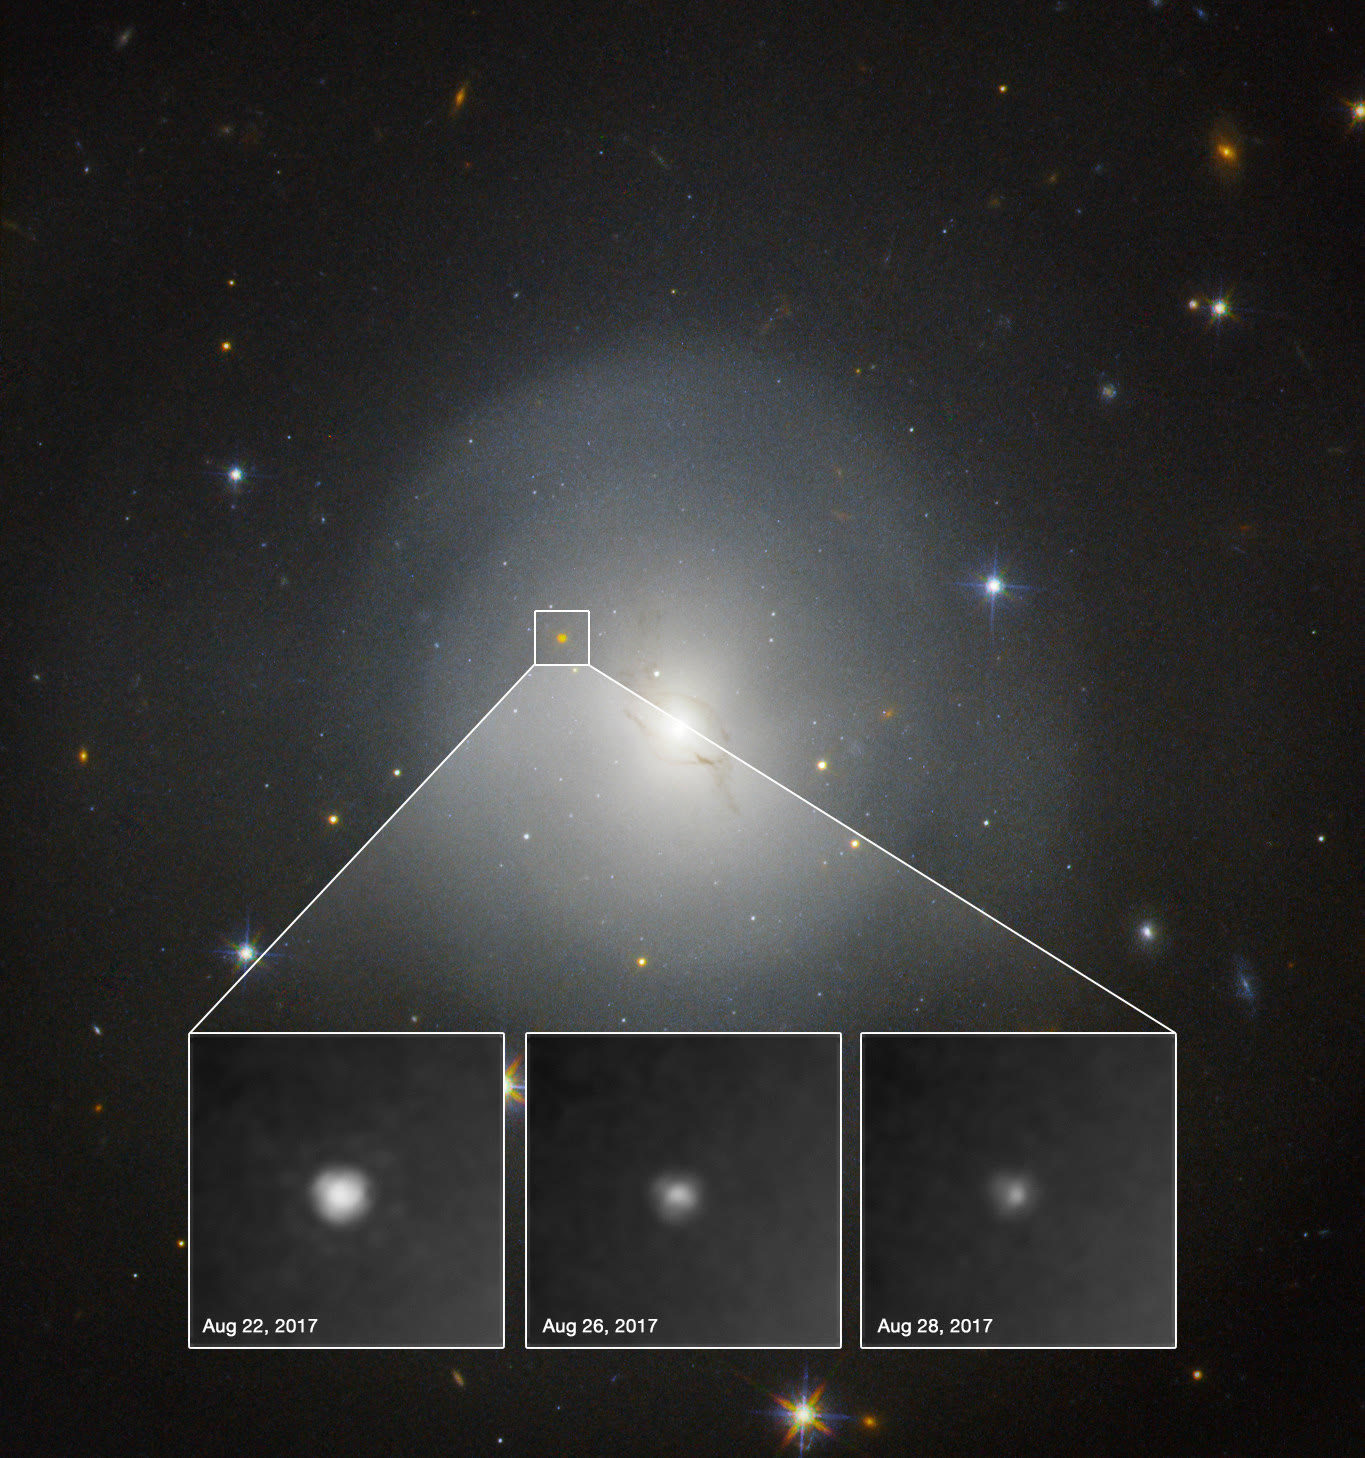
\includegraphics[width=0.55\linewidth]{images/book5/b3-kilonova.jpg}
\par\smallskip{\small A galáxia NGC~4993 fotografada pelo Hubble
Space Telescope após a coalescência de duas estrelas de nêutrons detectadas em
ondas gravitacionais em 17 de agosto de 2017. O retângulo marca a \omterm{def:b3:origin-of-elements:kilonova}{quilonova}; as
inserções, obtidas em 22, 26 e 28 de agosto, mostram seu enfraquecimento ao longo de seis dias.
NASA e ESA (A.~J.~Levan, N.~R.~Tanvir, A.~Fruchter e O.~Fox), CC
BY~4.0.}\label{fig:b3:origin-of-elements:kilonova}
\end{omfigure}
% ledger: photo:b3-kilonova

\begin{dated}{2021}
Não está estabelecido se as \omterm{def:b3:origin-of-elements:kilonova}{coalescências de estrelas de nêutrons} produzem a maior parte
dos elementos do \omterm{def:b3:origin-of-elements:s-process}{processo r} da Galáxia. As coalescências precisam esperar que suas órbitas
binárias decaiam, e os modelos da evolução da Galáxia em que elas são a única fonte
produzem os elementos do \omterm{def:b3:origin-of-elements:s-process}{processo r} tarde demais para explicar o que se vê nas
estrelas mais antigas e mais pobres em metais. Outras candidatas são os tipos raros de
supernova de colapso do núcleo, com rotação rápida e campos magnéticos intensos,
e o colapso de estrelas muito massivas; um modelo da Galáxia explica o európio observado
desde que cerca de três por cento das
hipernovas de 25 a \qty{50}{M_\odot} sejam do tipo impulsionado
magneticamente.
\end{dated}
% ledger: kobayashi20:origins, cowan21:rprocess

\section{A evolução química da Galáxia}\label{sec:b3:origin-of-elements:gce}

Cada geração de estrelas devolve ao gás parte do que produziu, e
a geração seguinte se forma a partir desse gás enriquecido. A composição de uma
estrela, portanto, registra a composição do gás no momento de seu nascimento, e as
estrelas de uma galáxia, ordenadas por idade, registram sua história.

\begin{definition}[Evolução química galáctica]\label{def:b3:origin-of-elements:gce}
A \emph{evolução química galáctica}\index{evolução química galáctica}
é a variação da composição do gás e das estrelas de uma galáxia ao longo do tempo,
sob a ação combinada da formação estelar, dos \omterm{def:b3:origin-of-elements:yield}{rendimentos estelares}, da duração
da vida das estrelas e do gás que entra na galáxia ou dela é expulso; e o estudo
dessa variação por meio de modelos comparados com as abundâncias de estrelas
de idade conhecida.
\end{definition}
% ledger: matteucci21:simple

O modelo mais simples trata uma região de uma galáxia como uma única caixa bem
misturada de gás, que se transforma lentamente em estrelas. Seja $s$ a massa retida em
estrelas de vida longa e em remanescentes estelares, $M_\mathrm{g}$ a massa de gás e
$M = M_\mathrm{g} + s$ o total. O \emph{rendimento por geração estelar} $y$ é a massa de
metais novos que uma geração de estrelas devolve ao gás
por unidade de massa que ela imobiliza.
% ledger: matteucci21:yield

\begin{theorem}[Modelo de caixa fechada]\label{thm:b3:origin-of-elements:closed-box}
\index{modelo de caixa fechada}
Considere uma região que não troca gás com o meio externo, começa como gás puro, sem metais,
se mantém bem misturada e na qual as estrelas que produzem metais morrem de imediato,
enquanto as demais vivem para sempre (reciclagem instantânea). Então, a \omterm{def:b3:origin-of-elements:metallicity}{metalicidade} do
gás é dada por
\[
Z = y \ln\frac{1}{\mu}, \qquad \mu = \frac{M_\mathrm{g}}{M},
\]
em que $\mu$ é a fração de gás e a massa de estrelas formadas com
\omterm{def:b3:origin-of-elements:metallicity}{metalicidade} abaixo de $Z$ é \mbox{$M\,(1 - \mathrm{e}^{-Z/y})$}.
\end{theorem}

\begin{proof}
Quando uma massa $\mathrm{d}s$ fica retida em estrelas, o gás perde
$\mathrm{d}s$, junto com os metais que contém, $Z\,\mathrm{d}s$,
e ganha $y\,\mathrm{d}s$ de metais novos:
$\mathrm{d}M_\mathrm{g} = -\mathrm{d}s$ e
$\mathrm{d}(Z M_\mathrm{g}) = (y - Z)\,\mathrm{d}s$. Desenvolvendo a
segunda, $M_\mathrm{g}\,\mathrm{d}Z + Z\,\mathrm{d}M_\mathrm{g} =
y\,\mathrm{d}s - Z\,\mathrm{d}s$, e os termos em $Z$ se cancelam:
$M_\mathrm{g}\,\mathrm{d}Z = -y\,\mathrm{d}M_\mathrm{g}$. Integrando
de $M_\mathrm{g} = M$, $Z = 0$ resulta $Z = y\ln(M/M_\mathrm{g})$. As
estrelas formadas enquanto a \omterm{def:b3:origin-of-elements:metallicity}{metalicidade} do gás estava abaixo de $Z$ são as formadas
enquanto o gás passava de $M$ para $M\mathrm{e}^{-Z/y}$, uma massa
$M(1 - \mathrm{e}^{-Z/y})$.
\end{proof}
% ledger: matteucci21:simple

O modelo prevê a distribuição de \omterm{def:b3:origin-of-elements:metallicity}{metalicidades} das estrelas de vida longa.
Na vizinhança solar, a densidade superficial de gás é
\qty{13.7}{M_\odot.pc^{-2}} e a de estrelas e remanescentes estelares
\qty{33.4}{M_\odot.pc^{-2}}, logo $\mu = 13.7/47.1 = 0.29$. Se o gás
hoje tem o $Z = 0.0154$ protossolar, o rendimento é
$y = 0.0154/\ln(1/0.29) = 0.0125$, e a fração de todas as estrelas
formadas até agora que têm $Z$ abaixo de um décimo do valor atual,
$[\mathrm{Fe/H}] < -1$ se o ferro acompanha os metais, é
$(1 - 0.29^{0.1})/(1 - 0.29) = 0.16$.
% ledger: mckee15:surface, asplund21:xyz, data:b5-gce

\begin{omfigure}
\centering
\begin{tikzpicture}
\begin{axis}[width=0.95\linewidth, height=7.2cm, xmin=-1.6, xmax=0.7,
  ymin=0, ymax=1500, xlabel={$[\mathrm{Fe/H}]$},
  ylabel={número de estrelas por \num{0.1}~dex},
  tick label style={font=\scriptsize}, label style={font=\small},
  legend style={font=\scriptsize, at={(0.5,-0.17)}, anchor=north,
    legend columns=3, draw=none, cells={anchor=west},
    /tikz/every even column/.append style={column sep=1em}}]
\addplot[ybar, area legend, bar width=0.085, fill=black!25, draw=black!50, bar shift=0pt]
  table[x=feh, y=n_obs] {figdata/out/bachelor-3-chemical_evolution-mdf.dat};
\addlegendentry{anãs F e G (6670)}
\addplot[ybar, area legend, bar width=0.085, fill=blue!55, draw=blue!70!black, bar shift=0pt]
  table[x=feh, y=n_low] {figdata/out/bachelor-3-chemical_evolution-mdf.dat};
\addlegendentry{no máximo \qty{1}{M_\odot} (902)}
\addplot[red!75!black, very thick, const plot mark mid]
  table[x=feh, y=model] {figdata/out/bachelor-3-chemical_evolution-mdf.dat};
\addlegendentry{caixa fechada}
\draw[black!50, dashed] (axis cs:-1,0) -- (axis cs:-1,1500);
\node[font=\scriptsize, anchor=north west, align=left] at (axis cs:-1.57,1450)
  {caixa fechada: \qty{16}{\percent}\\abaixo de $-1$;\\observado: \qty{0.4}{\percent}};
\end{axis}
\end{tikzpicture}
\par\smallskip{\small O \omterm{def:b3:origin-of-elements:g-dwarf}{problema das anãs G}. Barras: as \omterm{def:b3:origin-of-elements:metallicity}{metalicidades} das
anãs F e G da vizinhança solar (levantamento Genebra--Copenhague,
amostra de melhor fotometria reanalisada por Casagrande e outros, 2011), todas as
estrelas em cinza, as de no máximo uma massa solar, as estrelas de vida longa
que o modelo conta, em azul. Linha: a caixa fechada com a fração atual de gás
da vizinhança solar, reescalada para
o mesmo número de estrelas; ela não produz nenhuma estrela mais rica que seu gás atual,
tomado como solar. A caixa prevê uma longa cauda de estrelas pobres em metais
que não aparece.}\label{fig:b3:origin-of-elements:g-dwarf}
\end{omfigure}
% ledger: data:b5-gcs, casagrande11:gcs, data:b5-gce, mckee15:surface

\begin{definition}[Problema das anãs G]\label{def:b3:origin-of-elements:g-dwarf}
O \emph{problema das anãs G}\index{problema das anãs G} é a escassez de
estrelas de vida longa pobres em metais na vizinhança solar, em comparação com a
previsão do \omterm{thm:b3:origin-of-elements:closed-box}{modelo de caixa fechada}: bem menos das anãs de vida longa
de tipo espectral G têm \omterm{def:b3:origin-of-elements:metallicity}{metalicidade} baixa em número bem menor do que
uma caixa fechada teria produzido.
\end{definition}
% ledger: matteucci21:simple

Das 6670 estrelas da amostra do levantamento, 26 têm $[\mathrm{Fe/H}] < -1$:
\qty{0.4}{\percent}, contra os \qty{16}{\percent} da caixa fechada.
Mesmo entre as 902 estrelas de no máximo uma massa solar, a comparação mais justa,
as 26 representam \qty{2.9}{\percent}. A saída é abrir a
caixa: se o disco da vizinhança solar foi construído por uma lenta acreção
de gás pobre em metais ao longo de vários bilhões de anos, o gás inicial nunca foi
um grande reservatório à espera de formar estrelas pobres em metais, e a cauda
desaparece. Modelos do disco que reproduzem a distribuição exigem um
tempo de acreção maior que três a quatro bilhões de anos.
% ledger: data:b5-gcs, data:b5-gce, matteucci21:simple

O segundo relógio é a razão entre dois tipos de elemento. Os \omterm{def:b3:origin-of-elements:alpha}{elementos alfa}
vêm de supernovas de colapso de núcleo, logo após o nascimento de uma
geração estelar; grande parte do ferro vem de supernovas do tipo~Ia,
muito depois. Em estrelas antigas do halo, com $[\mathrm{Fe/H}] < -1$,
$[\alpha/\mathrm{Fe}]$ vale cerca de $+0.4$: essas estrelas se formaram a partir de gás
enriquecido apenas por supernovas de colapso de núcleo. Nas estrelas do disco, ela cai com
o aumento da \omterm{def:b3:origin-of-elements:metallicity}{metalicidade} até zero, o valor solar, à medida que as supernovas do tipo~Ia
somam seu ferro. A figura abaixo mostra o modelo mais simples
desse quadro de \emph{atraso temporal}: numa caixa fechada, os dois tipos de
supernova começam ao mesmo tempo, exceto que as do tipo~Ia começam com um atraso fixo
após as primeiras estrelas.
% ledger: matteucci21:time-delay, matteucci21:production

\begin{omfigure}
\centering
\begin{tikzpicture}
\begin{axis}[width=0.8\linewidth, height=6.4cm, xmin=-2.4, xmax=0.25,
  ymin=-0.08, ymax=0.55, xlabel={$[\mathrm{Fe/H}]$},
  ylabel={$[\alpha/\mathrm{Fe}]$},
  tick label style={font=\scriptsize}, label style={font=\small}]
\addplot[black!40, dashed, domain=-2.4:0.25, samples=2] {0};
\addplot[blue!70!black, very thick]
  table[x=feh, y=afe] {figdata/out/bachelor-3-chemical_evolution-alpha.dat};
\addplot[only marks, mark=*, mark size=2pt, red!70!black] coordinates {(-1,0.4) (0,0)};
\node[font=\scriptsize, anchor=south, align=center] at (axis cs:-1.75,0.41)
  {apenas supernovas de colapso de núcleo};
\node[font=\scriptsize, anchor=south west, align=left] at (axis cs:-0.98,0.41)
  {supernovas do tipo Ia\\[-1pt]começam};
\node[font=\scriptsize, anchor=south west] at (axis cs:0.01,0.01) {Sol};
\end{axis}
\end{tikzpicture}
\par\smallskip{\small Um modelo de duas fases de $[\alpha/\mathrm{Fe}]$ numa
caixa fechada: o platô em $+0.4$ é a razão produzida pelas supernovas de colapso de núcleo;
as supernovas do tipo~Ia, que começam quando o gás atinge
$[\mathrm{Fe/H}] = -1$, depois acrescentam ferro a uma taxa constante, até que a razão
seja solar em $[\mathrm{Fe/H}] = 0$. O platô e o joelho são os
observados nas estrelas da Galáxia; a forma entre eles é a do modelo.
Na \omterm{def:b3:origin-of-elements:metallicity}{metalicidade} do Sol, \qty{60}{\percent} do ferro neste modelo
veio de supernovas do tipo~Ia.}\label{fig:b3:origin-of-elements:alpha}
\end{omfigure}
% ledger: data:b5-gce, matteucci21:time-delay

Os modelos detalhados da Galáxia que reproduzem a tendência observada
atribuem dois terços do ferro às supernovas do tipo~Ia e um terço às
supernovas de colapso de núcleo, e concluem que o gás da Galáxia jovem
atingiu $[\mathrm{Fe/H}] = -1$ em cerca de um bilhão a um bilhão e meio
de anos. A razão é um relógio: uma população rica em \omterm{def:b3:origin-of-elements:alpha}{elementos alfa}
numa dada \omterm{def:b3:origin-of-elements:metallicity}{metalicidade} formou suas estrelas rapidamente, antes que as
supernovas do tipo~Ia pudessem somar seu ferro. O \omterm{def:b3:milky-way-galaxies:structure}{disco espesso} do
capítulo anterior é uma dessas populações: antiga, e levemente enriquecida
em \omterm{def:b3:origin-of-elements:alpha}{elementos alfa} em comparação com estrelas do disco fino de mesma \omterm{def:b3:origin-of-elements:metallicity}{metalicidade}.
% ledger: matteucci21:time-delay, casagrande11:gcs

\section{Das abundâncias solares à Terra}\label{sec:b3:origin-of-elements:earth}

A Terra é feita do mesmo material que o Sol, mas não de tudo o que é
dele. Na nebulosa em resfriamento, só os elementos que condensaram em sólidos
puderam ser reunidos em planetesimais; o volume do segundo ano seguiu a
sequência em que condensam. O ferro condensa como metal aproximadamente à
mesma temperatura que os silicatos de magnésio, \qtyrange{1310}{1340}{K} a
\qty{e-4}{bar}, de modo que os planetas rochosos ficaram com sua parte de ferro, enquanto
hidrogênio, hélio, carbono, nitrogênio e os gases nobres permaneceram no gás.
De um gás de composição solar, apenas cerca de meio por cento da massa
condensa como rocha e metal.
% ledger: lodders:tc-table, lodders:condensates

\begin{definition}[Tendência de volatilidade]\label{def:b3:origin-of-elements:volatility}
A \emph{tendência de volatilidade}\index{tendência de volatilidade} de um corpo planetário
é a diminuição de suas abundâncias, em relação aos condritos CI e
normalizadas por um elemento refratário, com a diminuição da temperatura de condensação
: elementos refratários permanecem nas suas proporções condríticas,
os moderadamente voláteis estão tanto mais empobrecidos quanto mais baixa for sua
temperatura de condensação.
\end{definition}

Para a Terra silicática, o volume do segundo ano traçou a tendência em função da
temperatura de condensação. Normalizado pelo magnésio, o zircônio
(condensa a \qty{1741}{K}) fica em \num{1.11} vezes a sua
proporção CI, o sódio (\qty{958}{K}) em \num{0.22}, o potássio
(\qty{1006}{K}) em \num{0.19}, o rubídio (\qty{800}{K}) em \num{0.12}
e o zinco (\qty{726}{K}) em \num{0.075}. A Terra se formou a partir de material
que já havia perdido parte de seus elementos moderadamente voláteis antes de
o planeta ser montado, ou os perdeu durante seu crescimento. Até os condritos CI
diferem do Sol de um modo que acompanha a temperatura de condensação,
embora de forma tênue: seus elementos moderadamente voláteis ficam
cerca de \num{0.04}~\omterm{def:b3:origin-of-elements:abundance}{dex} acima dos valores fotosféricos.
% ledger: lodders:tc-table, lodders:ci-table, ms95:pm-trace, asplund21:abstract

Assim, o registro deste capítulo atravessa o planeta. O oxigênio,
o magnésio e o silício do manto são \omterm{def:b3:origin-of-elements:alpha}{elementos alfa} de estrelas massivas;
o ferro do núcleo veio sobretudo de supernovas do tipo~Ia;
o tório e o urânio, cujo decaimento ajuda a aquecer o interior, situam-se além do
bismuto, onde só o \omterm{def:b3:origin-of-elements:s-process}{processo r} chega; e toda a mistura foi
separada por volatilidade antes que a Terra a reunisse.
% ledger: matteucci21:production, matteucci21:time-delay, kaeppeler11:overview, data:b5-sigman

\section*{Exercícios}

\begin{exercise}[$\star$]\label{exo:b3:origin-of-elements:1}
Use as \omterm{def:b3:origin-of-elements:abundance}{abundâncias solares} $\log\varepsilon(\mathrm{O}) = 8.69$,
$\log\varepsilon(\mathrm{Si}) = 7.51$, $\log\varepsilon(\mathrm{Fe}) =
7.46$, $\log\varepsilon(\mathrm{Au}) = 0.91$ e
$\log\varepsilon(\mathrm{Pb}) = 1.95$: (a)~quantos átomos de silício e
quantos átomos de oxigênio há no Sol por átomo de ferro? (b)~Quantos
átomos de ferro por átomo de ouro, e quantos átomos de chumbo por átomo de ouro?
\end{exercise}

\begin{exercise}[$\star$]\label{exo:b3:origin-of-elements:2}
(a)~Quantos átomos de ferro por milhão de átomos de hidrogênio contém o Sol
($\log\varepsilon(\mathrm{Fe}) = 7.46$)? (b)~Uma estrela do halo tem
$[\mathrm{Fe/H}] = -2$. Quantos átomos de hidrogênio ela contém por
átomo de ferro? (c)~Outra estrela tem um átomo de ferro para cada dez milhões
de átomos de hidrogênio. Qual é o seu $[\mathrm{Fe/H}]$?
\end{exercise}

\begin{exercise}[$\star$]\label{exo:b3:origin-of-elements:3}
Os isótopos estáveis do xenônio têm números de massa 124, 126, 128, 129, 130,
131, 132, 134 e 136. Entre seus isóbaros, o telúrio ($Z = 52$) tem
isótopos estáveis 120, 122--126, 128 e 130; o iodo ($Z = 53$) apenas 127.
O caminho s alcança o xenônio em $^{128}\mathrm{Xe}$, pelo decaimento de
$^{128}\mathrm{I}$, e dele sai em $^{133}\mathrm{Xe}$, que decai.
Classifique cada isótopo de xenônio como somente s, somente r, produzido
por ambos, ou núcleo p.
\end{exercise}

\begin{exercise}[$\star$]\label{exo:b3:origin-of-elements:4}
GW170817 situava-se a cerca de \qty{40}{Mpc}, e seus raios gama chegaram
\qty{1.7}{s} após a coalescência observada nas ondas gravitacionais. (a)~Há quanto tempo
os dois sinais viajavam? (b)~Se o atraso for atribuído inteiramente a uma
diferença entre as duas velocidades, qual é essa diferença como fração
da velocidade da luz, no máximo?
\end{exercise}

\begin{exercise}[$\star\star$]\label{exo:b3:origin-of-elements:5}
Os três isótopos de telúrio somente s têm abundâncias protossolares
\num{0.1067}, \num{0.0373} e \num{0.1984} por $10^6$ átomos de silício
($A = 122$, $123$, $124$) e seções de choque médias \num{295},
\num{832} e \qty{155}{mb}. (a)~Calcule $\sigma N$ para cada um. (b)~A partir
apenas do $^{122}\mathrm{Te}$, preveja as abundâncias de $^{123}\mathrm{Te}$
e de $^{124}\mathrm{Te}$, e compare. (c)~Por que a relação não pode ser
aplicada ao $^{128}\mathrm{Te}$?
\end{exercise}

\begin{exercise}[$\star\star$]\label{exo:b3:origin-of-elements:6}
No modelo clássico, cada núcleo no caminho s transfere ao seguinte uma fração
$f = 1/(1 + 1/(\tau_0\langle\sigma\rangle))$ do
fluxo, com $\tau_0 = \qty{0.306}{mb^{-1}}$. (a)~Calcule $f$ para
$^{124}\mathrm{Te}$ (\qty{155}{mb}) e para o
$^{138}\mathrm{Ba}$ de número de nêutrons mágico (\qty{4.0}{mb}). (b)~Os núcleos de
$^{137}\mathrm{Ba}$ a $^{142}\mathrm{Nd}$ no caminho têm seções de choque
\num{76.3}, \num{4.0}, \num{32.4}, \num{11.0},
\num{111.4} e \qty{35.0}{mb}. De que fator $\sigma N$ cai de
$^{136}\mathrm{Ba}$ até $^{142}\mathrm{Nd}$? (c)~Compare com os
valores medidos, \num{27.6} e \qty{7.72}{mb}.
\end{exercise}

\begin{exercise}[$\star\star$]\label{exo:b3:origin-of-elements:7}
Um nêutron de energia térmica $kT$ tem a velocidade
$v_T = \sqrt{2kT/m_\mathrm{n}}$, $m_\mathrm{n} = \qty{1.6749e-27}{kg}$.
(a)~Calcule $v_T$ para $kT = \qty{8}{keV}$, a temperatura da
camada de carbono-13 de uma gigante vermelha. (b)~Para o $^{124}\mathrm{Te}$, com
$\langle\sigma\rangle = \qty{155}{mb}$, calcule o tempo médio entre
duas capturas, $1/(n_\mathrm{n}\langle\sigma\rangle v_T)$, para
$n_\mathrm{n} = 10^6$, $10^8$ e \qty{e10}{cm^{-3}}. (c)~Compare com as
meias-vidas de $^{127}\mathrm{Te}$ (\qty{9.35}{h}) e de
$^{134}\mathrm{Cs}$ (\qty{2.07}{yr}). Qual deles é um ponto de ramificação?
\end{exercise}

\begin{exercise}[$\star\star$]\label{exo:b3:origin-of-elements:8}
No Sol, $\log\varepsilon$ é \num{6.30} para o cálcio, \num{3.14} para
o escândio e \num{4.97} para o titânio; \num{1.38} para o berílio,
\num{2.70} para o boro e \num{8.46} para o carbono. (a)~Quantas vezes
mais raro é o escândio do que seus dois vizinhos? (b)~Quantas vezes mais raro é
o berílio do que o carbono? (c)~Qual característica da curva
de abundância cada caso ilustra, e qual é a sua causa?
\end{exercise}

\begin{exercise}[$\star\star$]\label{exo:b3:origin-of-elements:9}
No modelo de duas fases do capítulo, o patamar
$[\alpha/\mathrm{Fe}] = P$ é a razão produzida pelas supernovas de colapso do núcleo,
e em $[\mathrm{Fe/H}] = 0$ a razão é solar. (a)~Mostre que a parcela do ferro
solar produzida por supernovas do tipo~Ia é $1 - 10^{-P}$, e
calcule-a para $P = 0.4$. (b)~Qual patamar daria os dois terços dos
modelos detalhados? (c)~Uma galáxia anã mostra seu joelho em
$[\mathrm{Fe/H}] = -2$. O que isso diz sobre a sua formação estelar?
\end{exercise}

\begin{exercise}[$\star\star\star$]\label{exo:b3:origin-of-elements:10}
As condritos CI contêm, em partes por milhão em massa, \num{95870}
de magnésio, \num{3.96} de zircônio, \num{5010} de sódio, \num{530}
de potássio e \num{2.13} de rubídio; a Terra silicática contém
\qty{22.8}{\percent} de magnésio e \num{10.5}, \num{2670}, \num{240}
e \num{0.6} partes por milhão dos demais. As temperaturas de condensação de 50 por cento
são \qty{1336}{K} (Mg), \qty{1741}{K} (Zr),
\qty{958}{K} (Na), \qty{1006}{K} (K) e \qty{800}{K} (Rb). (a)~Para
cada elemento calcule $(X/\mathrm{Mg})_\mathrm{Terra}/(X/\mathrm{Mg})_\mathrm{CI}$.
(b)~Represente-o em função da temperatura de condensação e descreva a
tendência. (c)~Por que o magnésio é escolhido como referência?
\end{exercise}

\begin{exercise}[$\star\star\star$]\label{exo:b3:origin-of-elements:11}
Uma caixa com vazamento perde gás em um vento a uma taxa $\lambda$ vezes
sua taxa de formação estelar, e não recebe nenhum. (a)~Mostre que sua \omterm{def:b3:origin-of-elements:metallicity}{metalicidade} é
$Z = \frac{y}{1 + \lambda}\ln\frac{M_\mathrm{g}(0)}{M_\mathrm{g}}$.
(b)~Com $y = 0.0125$, compare a \omterm{def:b3:origin-of-elements:metallicity}{metalicidade} atingida quando o gás caiu
para \qty{29}{\percent} de sua massa inicial, para $\lambda = 0$ e
$\lambda = 1$. (c)~Por que as galáxias pequenas, com gravidade fraca, tendem a
ser pobres em metais?
\end{exercise}

\begin{exercise}[$\star\star\star$]\label{exo:b3:origin-of-elements:12}
(a)~O Sol tem $\log\varepsilon(\mathrm{Li}) = 0.96$ em sua fotosfera
e os condritos CI têm $3.25$. Calcule as duas razões $N_\mathrm{Li}/N_\mathrm{H}$
e a fração do seu lítio que o Sol destruiu. (b)~As estrelas mais antigas pobres em metais
apresentam $N_\mathrm{Li}/N_\mathrm{H} = \num{1.45e-10}$,
enquanto a nucleossíntese do Big Bang prevê \num{4.72e-10}. Por qual fator
o lítio do Sistema Solar excede cada um deles? (c)~O que as duas
comparações implicam?
\end{exercise}

\section{Problema: uma galáxia de caixa fechada}

\begin{problem}[{Problema de fim de semana --- da mistura solar às
metalicidades das estrelas de vida longa}]
\label{pb:b3:origin-of-elements:1}
Use $\log\varepsilon(\mathrm{H}) = 12$, as \omterm{def:b3:origin-of-elements:abundance}{abundâncias solares}
$\log\varepsilon(\mathrm{Fe}) = 7.46$, $\log\varepsilon(\mathrm{O}) =
8.69$, $\log\varepsilon(\mathrm{He}) = 10.914$, as frações
mássicas fotosféricas atuais $X = 0.7438$, $Y = 0.2423$, $Z = 0.0139$,
e o $Z_\odot = 0.0154$ proto-solar. Suponha, ao longo de todo o problema, que o ferro
acompanha a \omterm{def:b3:origin-of-elements:metallicity}{metalicidade} total, $[\mathrm{Fe/H}] = \log_{10}(Z/Z_\odot)$.

\medskip\noindent\textbf{Parte I --- A mistura solar.}
\begin{enumerate}
\item Quantos átomos de hidrogênio existem no Sol por átomo de ferro?
\item Calcule a razão numérica $N_\mathrm{He}/N_\mathrm{H}$. Tomando
  um átomo de hélio quatro vezes mais pesado que um de hidrogênio, compare
  $4N_\mathrm{He}/N_\mathrm{H}$ com $Y/X$.
\item Uma estrela possui um átomo de ferro para cada \num{350000} átomos de hidrogênio.
  Calcule seu $[\mathrm{Fe/H}]$ com duas casas decimais.
\item A mesma estrela tem $[\mathrm{O/Fe}] = +0.40$. Calcule seu
  $\log\varepsilon(\mathrm{O})$ e o número de átomos de oxigênio por átomo de ferro,
  comparado com o do Sol.
\item O oxigênio é o metal mais abundante. Estime a fração mássica de metais da
  estrela escalonando a do Sol com $[\mathrm{O/H}]$.
\item Por que a \omterm{def:b3:origin-of-elements:metallicity}{metalicidade} de uma estrela costuma ser medida a partir do ferro
  e não a partir do oxigênio, embora este domine $Z$?
\end{enumerate}

\medskip\noindent\textbf{Parte II --- O processo s no telúrio.} Use
  os dados do \cref{exo:b3:origin-of-elements:5}.
\begin{enumerate}[resume]
\item Explique, a partir da carta de nuclídeos, por que $^{122}\mathrm{Te}$,
  $^{123}\mathrm{Te}$ e $^{124}\mathrm{Te}$ são somente do \omterm{def:b3:origin-of-elements:s-process}{processo s}.
\item Calcule $\sigma N$ para os três isótopos e para a sua média.
\item Preveja a abundância de $^{123}\mathrm{Te}$ a partir da média dos
  outros dois e dê a diferença em relação ao valor medido, em por
  cento.
\item $^{128}\mathrm{Te}$ tem $N = 1.329$ por $10^6$ Si e
  $\langle\sigma\rangle = \qty{44.4}{mb}$. Calcule seu $\sigma N$ e
  diga por que ele não está no patamar.
\item O par somente do \omterm{def:b3:origin-of-elements:s-process}{processo s} $^{148}\mathrm{Sm}$ e $^{150}\mathrm{Sm}$ tem
  $\sigma N = \num{7.43}$ e \qty{8.53}{mb}. Qual fração do fluxo
  contornou $^{148}\mathrm{Sm}$, e por qual ramificação?
\item Através de $N = 82$, o produto cai de \qty{27.6}{mb}
  ($^{136}\mathrm{Ba}$) para \qty{7.72}{mb} ($^{142}\mathrm{Nd}$). Qual
  propriedade dos núcleos com $N = 82$ explica a queda?
\end{enumerate}

\medskip\noindent\textbf{Parte III --- A caixa fechada.} A vizinhança solar
possui \qty{13.7}{M_\odot.pc^{-2}} de gás e
\qty{33.4}{M_\odot.pc^{-2}} de estrelas e remanescentes estelares. Tome o
gás atual com $Z = Z_\odot$.
\begin{enumerate}[resume]
\item Calcule a fração de gás atual $\mu_1$.
\item Calcule o rendimento por geração estelar $y$ que a caixa fechada
  exige, e sua razão com $Z_\odot$.
\item Calcule $Z$ e $[\mathrm{Fe/H}]$ do gás quando a fração de gás
  era $0.9$, depois $0.5$.
\item Calcule a fração de gás quando o gás atingiu
  $[\mathrm{Fe/H}] = -1$.
\item Qual fração da massa total havia então sido aprisionada em estrelas?
\item Se a fração de gás atual fosse $0.1$, qual rendimento a caixa
  exigiria?
\end{enumerate}

\medskip\noindent\textbf{Parte IV --- A distribuição de metalicidades.}
\begin{enumerate}[resume]
\item Mostre que a caixa fechada fornece uma distribuição de estrelas em
  $[\mathrm{Fe/H}]$ proporcional a $Z\,\mathrm{e}^{-Z/y}$, e encontre o
  $[\mathrm{Fe/H}]$ de seu pico.
\item Calcule a fração de todas as estrelas formadas até agora com
  $[\mathrm{Fe/H}] < -1$.
\item Calcule a fração com $[\mathrm{Fe/H}] < -0.5$.
\item Na amostra de levantamento de 6670 anãs F e G, 26 têm
  $[\mathrm{Fe/H}] < -1$. Quantas a caixa fechada prevê?
\item Entre as 902 estrelas de no máximo uma massa solar, encontram-se as
  mesmas 26. Calcule a fração observada e diga por que essa subamostra é
  a comparação mais justa.
\item Com uma fração de gás atual de $0.1$, qual seria a fração prevista
  abaixo de $-1$? Uma fração de gás diferente resolve o
  problema?
\item Forneça a fração de estrelas de vida longa com $[\mathrm{Fe/H}] < -1$
  que a caixa fechada prevê para a vizinhança solar, em por cento,
  com dois algarismos significativos, e diga o que a comparação com as
  estrelas observadas implica para a história do disco.
\end{enumerate}
\end{problem}
% ledger: asplund21:abstract, asplund21:xyz, data:b5-sigman, data:b5-kadonis, mckee15:surface, data:b5-gcs, data:b5-gce, matteucci21:simple
